% ============================================================================
% GRAPHICAL MODEL FIGURE: Knowledge Activation in LLMs
% ============================================================================
% Status: FINAL - Paper-ready TikZ figure
% Date: 2025-12-28
% Usage: % ============================================================================
% GRAPHICAL MODEL FIGURE: Knowledge Activation in LLMs
% ============================================================================
% Status: FINAL - Paper-ready TikZ figure
% Date: 2025-12-28
% Usage: % ============================================================================
% GRAPHICAL MODEL FIGURE: Knowledge Activation in LLMs
% ============================================================================
% Status: FINAL - Paper-ready TikZ figure
% Date: 2025-12-28
% Usage: % ============================================================================
% GRAPHICAL MODEL FIGURE: Knowledge Activation in LLMs
% ============================================================================
% Status: FINAL - Paper-ready TikZ figure
% Date: 2025-12-28
% Usage: \input{ESL_Graphical_Model_Figure.tex} or standalone compilation
% ============================================================================

\documentclass[11pt,a4paper]{article}
\usepackage[utf8]{inputenc}
\usepackage[T1]{fontenc}
\usepackage{amsmath,amssymb}
\usepackage{tikz}
\usetikzlibrary{arrows.meta,positioning,shapes.geometric,calc,decorations.pathmorphing}
\usepackage[margin=1in]{geometry}

\title{\textbf{Graphical Model: Knowledge Activation in LLMs}}
\author{BEATRIX Research Group}
\date{December 2025}

\begin{document}
\maketitle

% ============================================================================
\section{Main Figure: The Activation Gap}
% ============================================================================

\begin{figure}[h]
\centering
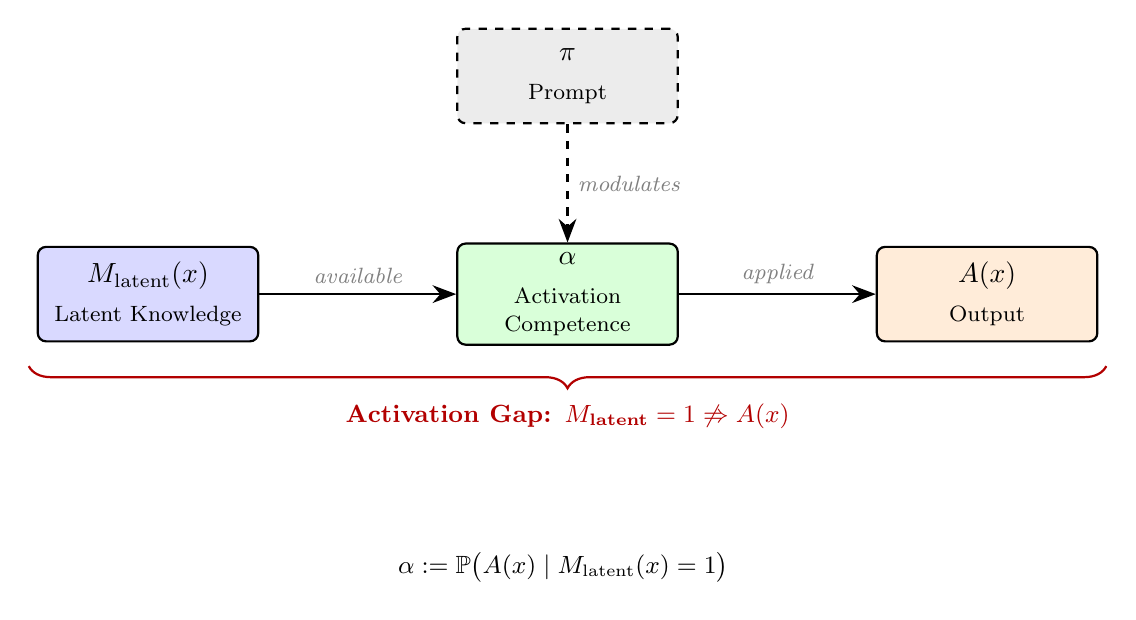
\begin{tikzpicture}[
    node distance=2.5cm,
    box/.style={rectangle, draw=black, thick, minimum width=2.8cm, minimum height=1.2cm, align=center, rounded corners=3pt},
    latent/.style={box, fill=blue!15},
    activation/.style={box, fill=green!15},
    output/.style={box, fill=orange!15},
    prompt/.style={box, fill=gray!15, dashed},
    arrow/.style={-{Stealth[length=3mm]}, thick},
    label/.style={font=\footnotesize\itshape, text=gray}
]

% Main pathway
\node[latent] (M) {$M_{\text{latent}}(x)$\\[2pt]\footnotesize Latent Knowledge};
\node[activation, right=of M] (alpha) {$\alpha$\\[2pt]\footnotesize Activation\\[-2pt]\footnotesize Competence};
\node[output, right=of alpha] (A) {$A(x)$\\[2pt]\footnotesize Output};

% Prompt node (influencing activation)
\node[prompt, above=1.5cm of alpha] (pi) {$\pi$\\[2pt]\footnotesize Prompt};

% Arrows
\draw[arrow] (M) -- (alpha) node[midway, above, label] {available};
\draw[arrow] (alpha) -- (A) node[midway, above, label] {applied};
\draw[arrow, dashed] (pi) -- (alpha) node[midway, right, label] {modulates};

% The Gap annotation
\draw[decorate, decoration={brace, amplitude=8pt, mirror}, thick, red!70!black]
    ($(M.south west)+(-0.1,-0.3)$) -- ($(A.south east)+(0.1,-0.3)$)
    node[midway, below=10pt, text=red!70!black, font=\small\bfseries] {Activation Gap: $M_{\text{latent}} = 1 \not\Rightarrow A(x)$};

% Probability annotation
\node[below=2.5cm of alpha, align=center, font=\small] {
    $\alpha := \mathbb{P}\big(A(x) \mid M_{\text{latent}}(x) = 1\big)$
};

\end{tikzpicture}
\caption{\textbf{The Knowledge Activation Model.} Latent knowledge $M_{\text{latent}}$ must pass through activation competence $\alpha$ before manifesting as correct output $A(x)$. The prompt $\pi$ modulates $\alpha$ but cannot create knowledge. The \textcolor{red!70!black}{activation gap} represents the central finding: knowledge availability does not imply knowledge use.}
\label{fig:activation-model}
\end{figure}


% ============================================================================
\section{Extended Figure: Decomposition and Prompt Effects}
% ============================================================================

\begin{figure}[h]
\centering
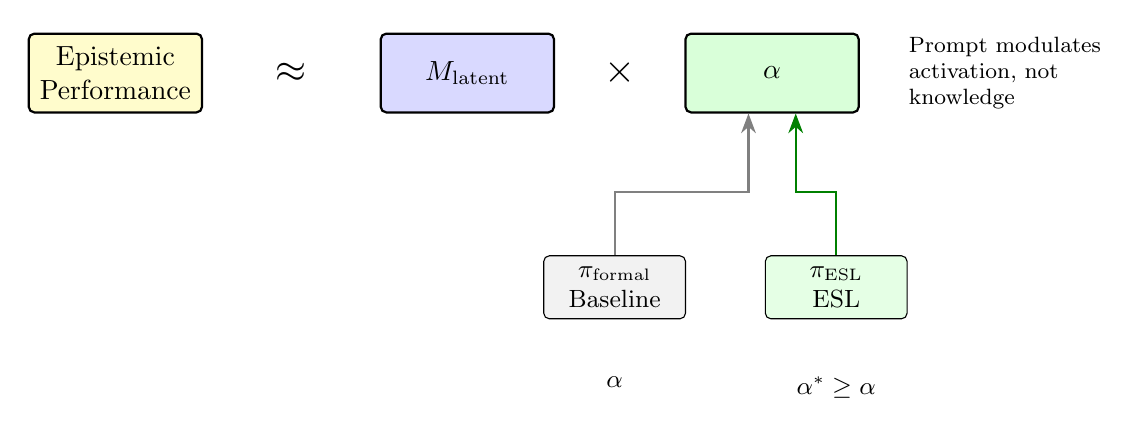
\begin{tikzpicture}[
    node distance=2cm,
    box/.style={rectangle, draw=black, thick, minimum width=2.2cm, minimum height=1cm, align=center, rounded corners=2pt},
    small/.style={rectangle, draw=black, minimum width=1.8cm, minimum height=0.8cm, align=center, rounded corners=2pt, font=\small},
    arrow/.style={-{Stealth[length=2.5mm]}, thick},
    eq/.style={font=\Large}
]

% Performance decomposition
\node[box, fill=yellow!20] (perf) {Epistemic\\Performance};
\node[eq, right=0.8cm of perf] (eq1) {$\approx$};
\node[box, fill=blue!15, right=0.8cm of eq1] (M2) {$M_{\text{latent}}$};
\node[eq, right=0.5cm of M2] (times) {$\times$};
\node[box, fill=green!15, right=0.5cm of times] (alpha2) {$\alpha$};

% Prompt conditions below
\node[small, fill=gray!10, below=1.8cm of alpha2, xshift=-2cm] (baseline) {$\pi_{\text{formal}}$\\Baseline};
\node[small, fill=green!10, right=1cm of baseline] (esl) {$\pi_{\text{ESL}}$\\ESL};

% Alpha values
\node[below=0.6cm of baseline, font=\small] (a1) {$\alpha$};
\node[below=0.6cm of esl, font=\small] (a2) {$\alpha^* \geq \alpha$};

% Arrows from prompts to alpha
\draw[arrow, gray] (baseline.north) -- ++(0,0.8) -| ($(alpha2.south)+(-0.3,0)$);
\draw[arrow, green!50!black] (esl.north) -- ++(0,0.8) -| ($(alpha2.south)+(0.3,0)$);

% Annotation
\node[right=0.5cm of alpha2, align=left, font=\footnotesize] {
    Prompt modulates\\
    activation, not\\
    knowledge
};

\end{tikzpicture}
\caption{\textbf{Performance Decomposition.} Epistemic performance decomposes into latent knowledge times activation competence. Different prompts ($\pi_{\text{formal}}$ vs.\ $\pi_{\text{ESL}}$) yield different activation levels, with ESL achieving $\alpha^* \geq \alpha$.}
\label{fig:decomposition}
\end{figure}


% ============================================================================
\section{Comparative Figure: Model Profiles}
% ============================================================================

\begin{figure}[h]
\centering
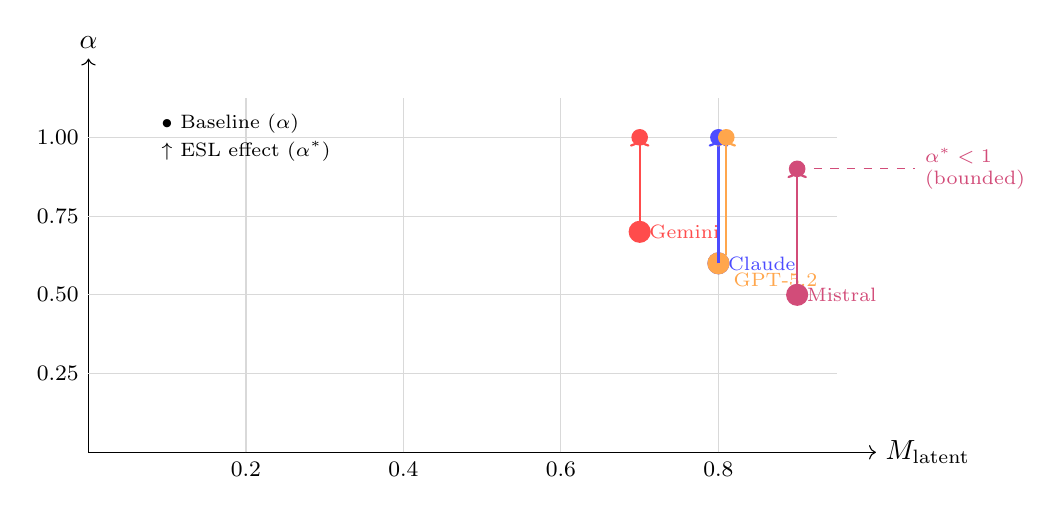
\begin{tikzpicture}[
    bar/.style={thick},
    label/.style={font=\footnotesize}
]

% Axes
\draw[->] (0,0) -- (10,0) node[right] {$M_{\text{latent}}$};
\draw[->] (0,0) -- (0,5) node[above] {$\alpha$};

% Grid
\foreach \x in {2,4,6,8} {
    \draw[gray!30] (\x,0) -- (\x,4.5);
}
\foreach \y in {1,2,3,4} {
    \draw[gray!30] (0,\y) -- (9.5,\y);
}

% Axis labels
\node[label, below] at (2,0) {0.2};
\node[label, below] at (4,0) {0.4};
\node[label, below] at (6,0) {0.6};
\node[label, below] at (8,0) {0.8};
\node[label, left] at (0,1) {0.25};
\node[label, left] at (0,2) {0.50};
\node[label, left] at (0,3) {0.75};
\node[label, left] at (0,4) {1.00};

% Model points (Baseline)
\fill[blue!70] (8,2.4) circle (4pt) node[right, font=\scriptsize] {Claude};
\fill[red!70] (7,2.8) circle (4pt) node[right, font=\scriptsize] {Gemini};
\fill[orange!70] (8,2.4) circle (4pt) node[below right, font=\scriptsize, xshift=2pt] {GPT-5.2};
\fill[purple!70] (9,2) circle (4pt) node[right, font=\scriptsize] {Mistral};

% Arrows to ESL positions
\draw[->, blue!70, thick] (8,2.4) -- (8,4);
\draw[->, red!70, thick] (7,2.8) -- (7,4);
\draw[->, orange!70, thick] (8.1,2.5) -- (8.1,4);
\draw[->, purple!70, thick] (9,2) -- (9,3.6);

% ESL points
\fill[blue!70] (8,4) circle (3pt);
\fill[red!70] (7,4) circle (3pt);
\fill[orange!70] (8.1,4) circle (3pt);
\fill[purple!70] (9,3.6) circle (3pt);

% Legend
\node[font=\scriptsize, align=left] at (2,4) {
    $\bullet$ Baseline ($\alpha$)\\[2pt]
    $\uparrow$ ESL effect ($\alpha^*$)
};

% Annotation for Mistral
\draw[purple!70, dashed] (9,3.6) -- (10.5,3.6) node[right, font=\scriptsize, align=left] {$\alpha^* < 1$\\(bounded)};

\end{tikzpicture}
\caption{\textbf{Cross-Model Activation Profiles.} All models have high latent knowledge ($M_{\text{latent}} \approx 0.8$--$0.9$), but vary in baseline activation ($\alpha = 0.50$--$0.70$). ESL prompting increases $\alpha$ to $\alpha^*$, with most models reaching 1.00. Mistral shows bounded activation ($\alpha^* = 0.90 < 1$), indicating intrinsic limitations.}
\label{fig:model-profiles}
\end{figure}


% ============================================================================
\section{Conceptual Figure: Hallucination as Activation Failure}
% ============================================================================

\begin{figure}[h]
\centering
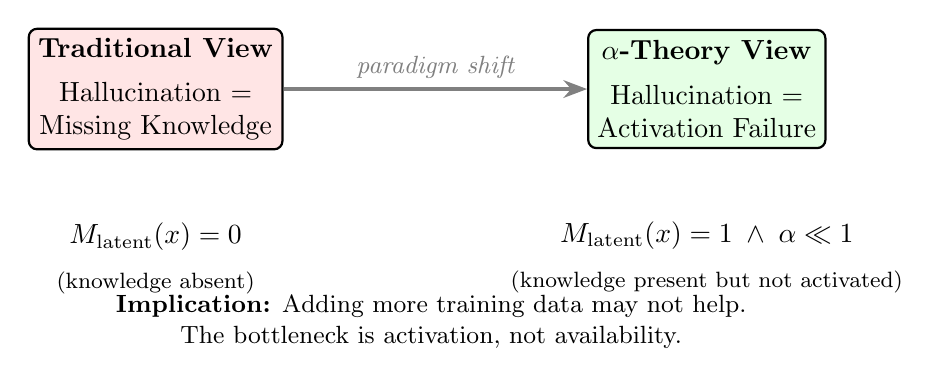
\begin{tikzpicture}[
    box/.style={rectangle, draw=black, thick, minimum width=3cm, minimum height=1.5cm, align=center, rounded corners=3pt},
    arrow/.style={-{Stealth[length=3mm]}, thick}
]

% Two scenarios side by side
% Scenario 1: Traditional view
\node[box, fill=red!10] (trad) at (0,0) {\textbf{Traditional View}\\[4pt]Hallucination =\\Missing Knowledge};

% Scenario 2: Alpha view
\node[box, fill=green!10] (alpha) at (7,0) {\textbf{$\alpha$-Theory View}\\[4pt]Hallucination =\\Activation Failure};

% Formulas below
\node[below=0.8cm of trad, align=center] {
    $M_{\text{latent}}(x) = 0$\\[4pt]
    \footnotesize (knowledge absent)
};

\node[below=0.8cm of alpha, align=center] {
    $M_{\text{latent}}(x) = 1 \;\land\; \alpha \ll 1$\\[4pt]
    \footnotesize (knowledge present but not activated)
};

% Arrow between views
\draw[arrow, very thick, gray] (trad) -- (alpha) node[midway, above, font=\small\itshape] {paradigm shift};

% Implication
\node[below=2.5cm of $(trad)!0.5!(alpha)$, align=center, font=\small] {
    \textbf{Implication:} Adding more training data may not help.\\
    The bottleneck is activation, not availability.
};

\end{tikzpicture}
\caption{\textbf{Reframing Hallucination.} The traditional view attributes hallucination to missing knowledge. The $\alpha$-theory reframes it as activation failure: the model possesses the relevant knowledge but fails to apply it during generation.}
\label{fig:hallucination-reframe}
\end{figure}


% ============================================================================
\section{Paper-Ready Single Figure (Recommended for Main Text)}
% ============================================================================

\begin{figure}[h]
\centering
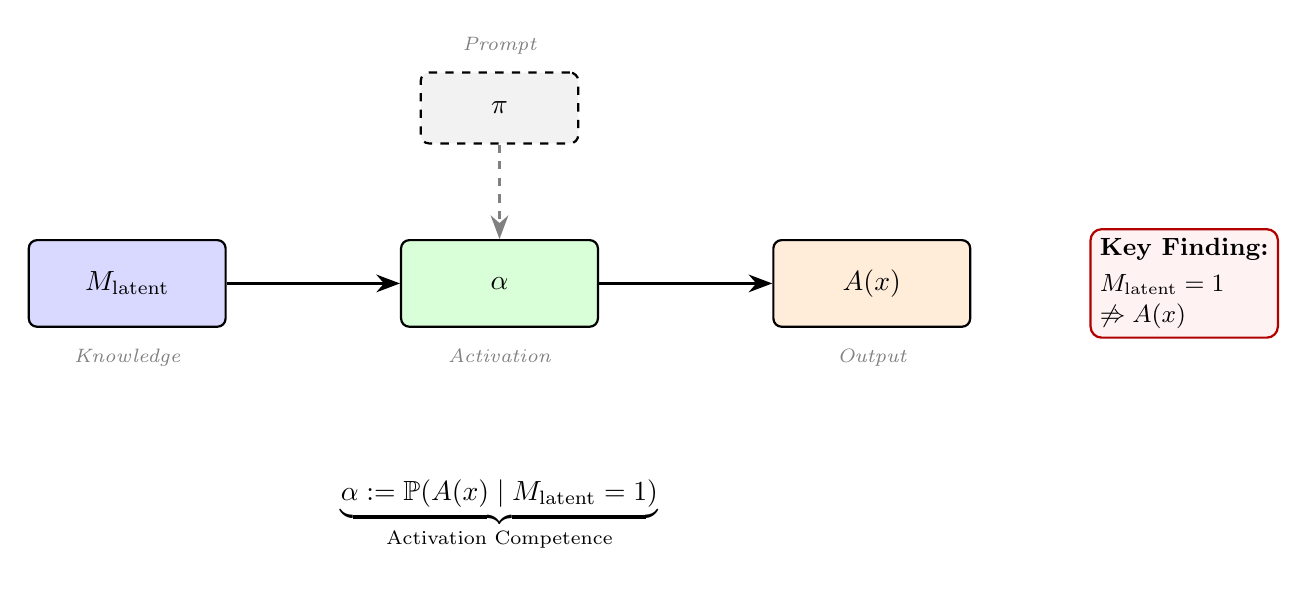
\begin{tikzpicture}[
    node distance=2.2cm,
    main/.style={rectangle, draw=black, thick, minimum width=2.5cm, minimum height=1.1cm, align=center, rounded corners=3pt},
    prompt/.style={rectangle, draw=black, thick, dashed, minimum width=2cm, minimum height=0.9cm, align=center, rounded corners=3pt, fill=gray!10},
    arrow/.style={-{Stealth[length=3mm]}, thick},
    note/.style={font=\scriptsize\itshape, text=gray}
]

% Main flow
\node[main, fill=blue!15] (M) {$M_{\text{latent}}$};
\node[main, fill=green!15, right=of M] (alpha) {$\alpha$};
\node[main, fill=orange!15, right=of alpha] (A) {$A(x)$};

% Prompt
\node[prompt, above=1.2cm of alpha] (pi) {$\pi$};

% Arrows
\draw[arrow] (M) -- (alpha);
\draw[arrow] (alpha) -- (A);
\draw[arrow, dashed, gray] (pi) -- (alpha);

% Labels
\node[note, below=0.15cm of M] {Knowledge};
\node[note, below=0.15cm of alpha] {Activation};
\node[note, below=0.15cm of A] {Output};
\node[note, above=0.1cm of pi] {Prompt};

% Equation
\node[below=1.8cm of alpha] {
    $\underbrace{\alpha := \mathbb{P}(A(x) \mid M_{\text{latent}} = 1)}_{\text{Activation Competence}}$
};

% Key insight box
\node[draw=red!70!black, thick, rounded corners, fill=red!5,
      right=1.5cm of A, align=left, font=\small] (insight) {
    \textbf{Key Finding:}\\[2pt]
    $M_{\text{latent}} = 1$\\
    $\not\Rightarrow A(x)$
};

\end{tikzpicture}
\caption{\textbf{Knowledge Activation Model.} The path from latent knowledge ($M_{\text{latent}}$) to correct output ($A(x)$) is mediated by activation competence ($\alpha$). Prompts ($\pi$) can modulate $\alpha$ but cannot create knowledge. The central finding is that knowledge availability does not guarantee knowledge application.}
\label{fig:main-model}
\end{figure}


% ============================================================================
% USAGE NOTES
% ============================================================================
%
% For paper inclusion, use Figure 5 (fig:main-model) as the main text figure.
% Other figures can go in appendix or supplementary material.
%
% Required packages:
% \usepackage{tikz}
% \usetikzlibrary{arrows.meta,positioning,shapes.geometric,calc,decorations.pathmorphing}
%
% To include in main paper:
% \begin{figure}[t]
%   \centering
%   \input{figures/activation-model.tikz}
%   \caption{...}
% \end{figure}
%

\end{document}
 or standalone compilation
% ============================================================================

\documentclass[11pt,a4paper]{article}
\usepackage[utf8]{inputenc}
\usepackage[T1]{fontenc}
\usepackage{amsmath,amssymb}
\usepackage{tikz}
\usetikzlibrary{arrows.meta,positioning,shapes.geometric,calc,decorations.pathmorphing}
\usepackage[margin=1in]{geometry}

\title{\textbf{Graphical Model: Knowledge Activation in LLMs}}
\author{BEATRIX Research Group}
\date{December 2025}

\begin{document}
\maketitle

% ============================================================================
\section{Main Figure: The Activation Gap}
% ============================================================================

\begin{figure}[h]
\centering
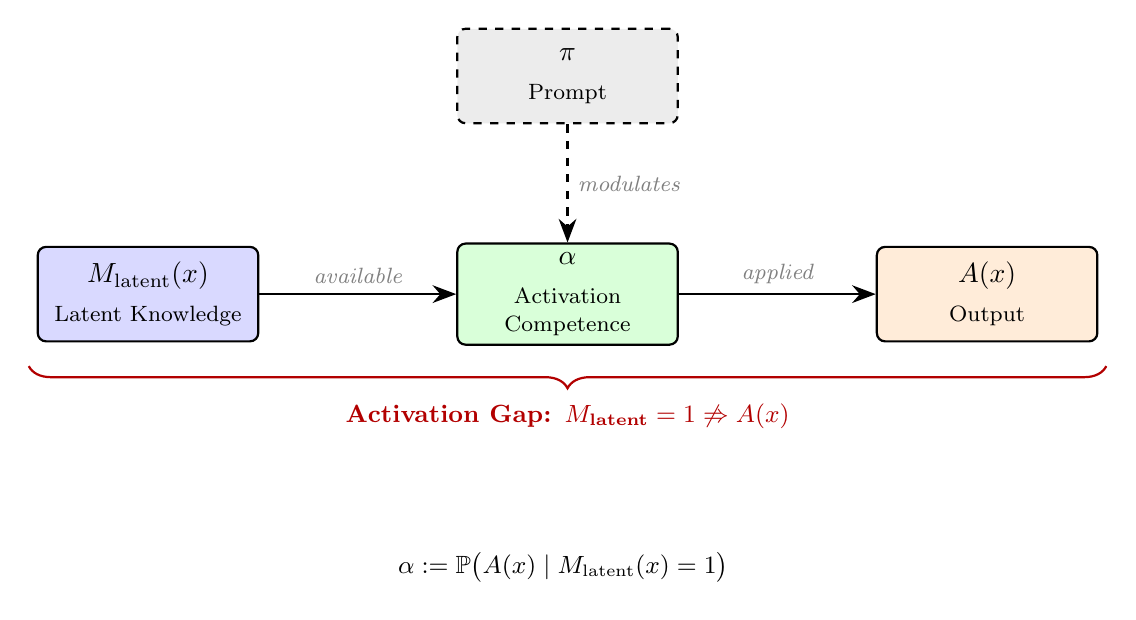
\begin{tikzpicture}[
    node distance=2.5cm,
    box/.style={rectangle, draw=black, thick, minimum width=2.8cm, minimum height=1.2cm, align=center, rounded corners=3pt},
    latent/.style={box, fill=blue!15},
    activation/.style={box, fill=green!15},
    output/.style={box, fill=orange!15},
    prompt/.style={box, fill=gray!15, dashed},
    arrow/.style={-{Stealth[length=3mm]}, thick},
    label/.style={font=\footnotesize\itshape, text=gray}
]

% Main pathway
\node[latent] (M) {$M_{\text{latent}}(x)$\\[2pt]\footnotesize Latent Knowledge};
\node[activation, right=of M] (alpha) {$\alpha$\\[2pt]\footnotesize Activation\\[-2pt]\footnotesize Competence};
\node[output, right=of alpha] (A) {$A(x)$\\[2pt]\footnotesize Output};

% Prompt node (influencing activation)
\node[prompt, above=1.5cm of alpha] (pi) {$\pi$\\[2pt]\footnotesize Prompt};

% Arrows
\draw[arrow] (M) -- (alpha) node[midway, above, label] {available};
\draw[arrow] (alpha) -- (A) node[midway, above, label] {applied};
\draw[arrow, dashed] (pi) -- (alpha) node[midway, right, label] {modulates};

% The Gap annotation
\draw[decorate, decoration={brace, amplitude=8pt, mirror}, thick, red!70!black]
    ($(M.south west)+(-0.1,-0.3)$) -- ($(A.south east)+(0.1,-0.3)$)
    node[midway, below=10pt, text=red!70!black, font=\small\bfseries] {Activation Gap: $M_{\text{latent}} = 1 \not\Rightarrow A(x)$};

% Probability annotation
\node[below=2.5cm of alpha, align=center, font=\small] {
    $\alpha := \mathbb{P}\big(A(x) \mid M_{\text{latent}}(x) = 1\big)$
};

\end{tikzpicture}
\caption{\textbf{The Knowledge Activation Model.} Latent knowledge $M_{\text{latent}}$ must pass through activation competence $\alpha$ before manifesting as correct output $A(x)$. The prompt $\pi$ modulates $\alpha$ but cannot create knowledge. The \textcolor{red!70!black}{activation gap} represents the central finding: knowledge availability does not imply knowledge use.}
\label{fig:activation-model}
\end{figure}


% ============================================================================
\section{Extended Figure: Decomposition and Prompt Effects}
% ============================================================================

\begin{figure}[h]
\centering
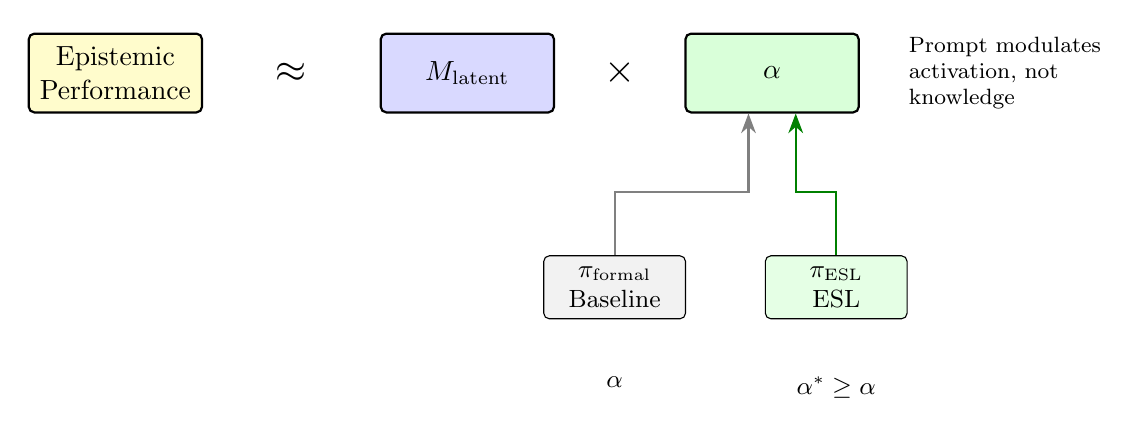
\begin{tikzpicture}[
    node distance=2cm,
    box/.style={rectangle, draw=black, thick, minimum width=2.2cm, minimum height=1cm, align=center, rounded corners=2pt},
    small/.style={rectangle, draw=black, minimum width=1.8cm, minimum height=0.8cm, align=center, rounded corners=2pt, font=\small},
    arrow/.style={-{Stealth[length=2.5mm]}, thick},
    eq/.style={font=\Large}
]

% Performance decomposition
\node[box, fill=yellow!20] (perf) {Epistemic\\Performance};
\node[eq, right=0.8cm of perf] (eq1) {$\approx$};
\node[box, fill=blue!15, right=0.8cm of eq1] (M2) {$M_{\text{latent}}$};
\node[eq, right=0.5cm of M2] (times) {$\times$};
\node[box, fill=green!15, right=0.5cm of times] (alpha2) {$\alpha$};

% Prompt conditions below
\node[small, fill=gray!10, below=1.8cm of alpha2, xshift=-2cm] (baseline) {$\pi_{\text{formal}}$\\Baseline};
\node[small, fill=green!10, right=1cm of baseline] (esl) {$\pi_{\text{ESL}}$\\ESL};

% Alpha values
\node[below=0.6cm of baseline, font=\small] (a1) {$\alpha$};
\node[below=0.6cm of esl, font=\small] (a2) {$\alpha^* \geq \alpha$};

% Arrows from prompts to alpha
\draw[arrow, gray] (baseline.north) -- ++(0,0.8) -| ($(alpha2.south)+(-0.3,0)$);
\draw[arrow, green!50!black] (esl.north) -- ++(0,0.8) -| ($(alpha2.south)+(0.3,0)$);

% Annotation
\node[right=0.5cm of alpha2, align=left, font=\footnotesize] {
    Prompt modulates\\
    activation, not\\
    knowledge
};

\end{tikzpicture}
\caption{\textbf{Performance Decomposition.} Epistemic performance decomposes into latent knowledge times activation competence. Different prompts ($\pi_{\text{formal}}$ vs.\ $\pi_{\text{ESL}}$) yield different activation levels, with ESL achieving $\alpha^* \geq \alpha$.}
\label{fig:decomposition}
\end{figure}


% ============================================================================
\section{Comparative Figure: Model Profiles}
% ============================================================================

\begin{figure}[h]
\centering
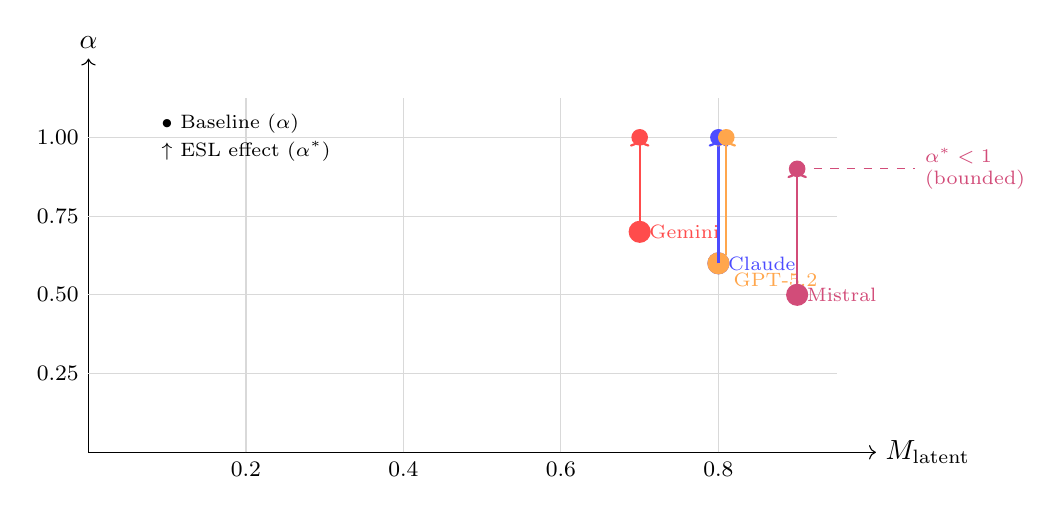
\begin{tikzpicture}[
    bar/.style={thick},
    label/.style={font=\footnotesize}
]

% Axes
\draw[->] (0,0) -- (10,0) node[right] {$M_{\text{latent}}$};
\draw[->] (0,0) -- (0,5) node[above] {$\alpha$};

% Grid
\foreach \x in {2,4,6,8} {
    \draw[gray!30] (\x,0) -- (\x,4.5);
}
\foreach \y in {1,2,3,4} {
    \draw[gray!30] (0,\y) -- (9.5,\y);
}

% Axis labels
\node[label, below] at (2,0) {0.2};
\node[label, below] at (4,0) {0.4};
\node[label, below] at (6,0) {0.6};
\node[label, below] at (8,0) {0.8};
\node[label, left] at (0,1) {0.25};
\node[label, left] at (0,2) {0.50};
\node[label, left] at (0,3) {0.75};
\node[label, left] at (0,4) {1.00};

% Model points (Baseline)
\fill[blue!70] (8,2.4) circle (4pt) node[right, font=\scriptsize] {Claude};
\fill[red!70] (7,2.8) circle (4pt) node[right, font=\scriptsize] {Gemini};
\fill[orange!70] (8,2.4) circle (4pt) node[below right, font=\scriptsize, xshift=2pt] {GPT-5.2};
\fill[purple!70] (9,2) circle (4pt) node[right, font=\scriptsize] {Mistral};

% Arrows to ESL positions
\draw[->, blue!70, thick] (8,2.4) -- (8,4);
\draw[->, red!70, thick] (7,2.8) -- (7,4);
\draw[->, orange!70, thick] (8.1,2.5) -- (8.1,4);
\draw[->, purple!70, thick] (9,2) -- (9,3.6);

% ESL points
\fill[blue!70] (8,4) circle (3pt);
\fill[red!70] (7,4) circle (3pt);
\fill[orange!70] (8.1,4) circle (3pt);
\fill[purple!70] (9,3.6) circle (3pt);

% Legend
\node[font=\scriptsize, align=left] at (2,4) {
    $\bullet$ Baseline ($\alpha$)\\[2pt]
    $\uparrow$ ESL effect ($\alpha^*$)
};

% Annotation for Mistral
\draw[purple!70, dashed] (9,3.6) -- (10.5,3.6) node[right, font=\scriptsize, align=left] {$\alpha^* < 1$\\(bounded)};

\end{tikzpicture}
\caption{\textbf{Cross-Model Activation Profiles.} All models have high latent knowledge ($M_{\text{latent}} \approx 0.8$--$0.9$), but vary in baseline activation ($\alpha = 0.50$--$0.70$). ESL prompting increases $\alpha$ to $\alpha^*$, with most models reaching 1.00. Mistral shows bounded activation ($\alpha^* = 0.90 < 1$), indicating intrinsic limitations.}
\label{fig:model-profiles}
\end{figure}


% ============================================================================
\section{Conceptual Figure: Hallucination as Activation Failure}
% ============================================================================

\begin{figure}[h]
\centering
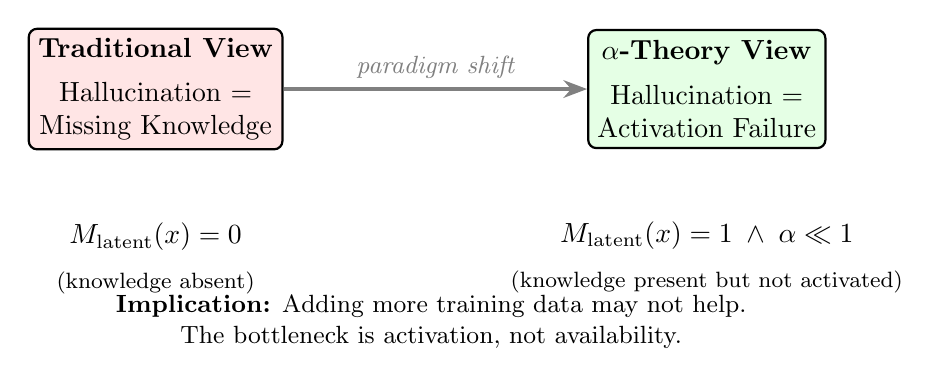
\begin{tikzpicture}[
    box/.style={rectangle, draw=black, thick, minimum width=3cm, minimum height=1.5cm, align=center, rounded corners=3pt},
    arrow/.style={-{Stealth[length=3mm]}, thick}
]

% Two scenarios side by side
% Scenario 1: Traditional view
\node[box, fill=red!10] (trad) at (0,0) {\textbf{Traditional View}\\[4pt]Hallucination =\\Missing Knowledge};

% Scenario 2: Alpha view
\node[box, fill=green!10] (alpha) at (7,0) {\textbf{$\alpha$-Theory View}\\[4pt]Hallucination =\\Activation Failure};

% Formulas below
\node[below=0.8cm of trad, align=center] {
    $M_{\text{latent}}(x) = 0$\\[4pt]
    \footnotesize (knowledge absent)
};

\node[below=0.8cm of alpha, align=center] {
    $M_{\text{latent}}(x) = 1 \;\land\; \alpha \ll 1$\\[4pt]
    \footnotesize (knowledge present but not activated)
};

% Arrow between views
\draw[arrow, very thick, gray] (trad) -- (alpha) node[midway, above, font=\small\itshape] {paradigm shift};

% Implication
\node[below=2.5cm of $(trad)!0.5!(alpha)$, align=center, font=\small] {
    \textbf{Implication:} Adding more training data may not help.\\
    The bottleneck is activation, not availability.
};

\end{tikzpicture}
\caption{\textbf{Reframing Hallucination.} The traditional view attributes hallucination to missing knowledge. The $\alpha$-theory reframes it as activation failure: the model possesses the relevant knowledge but fails to apply it during generation.}
\label{fig:hallucination-reframe}
\end{figure}


% ============================================================================
\section{Paper-Ready Single Figure (Recommended for Main Text)}
% ============================================================================

\begin{figure}[h]
\centering
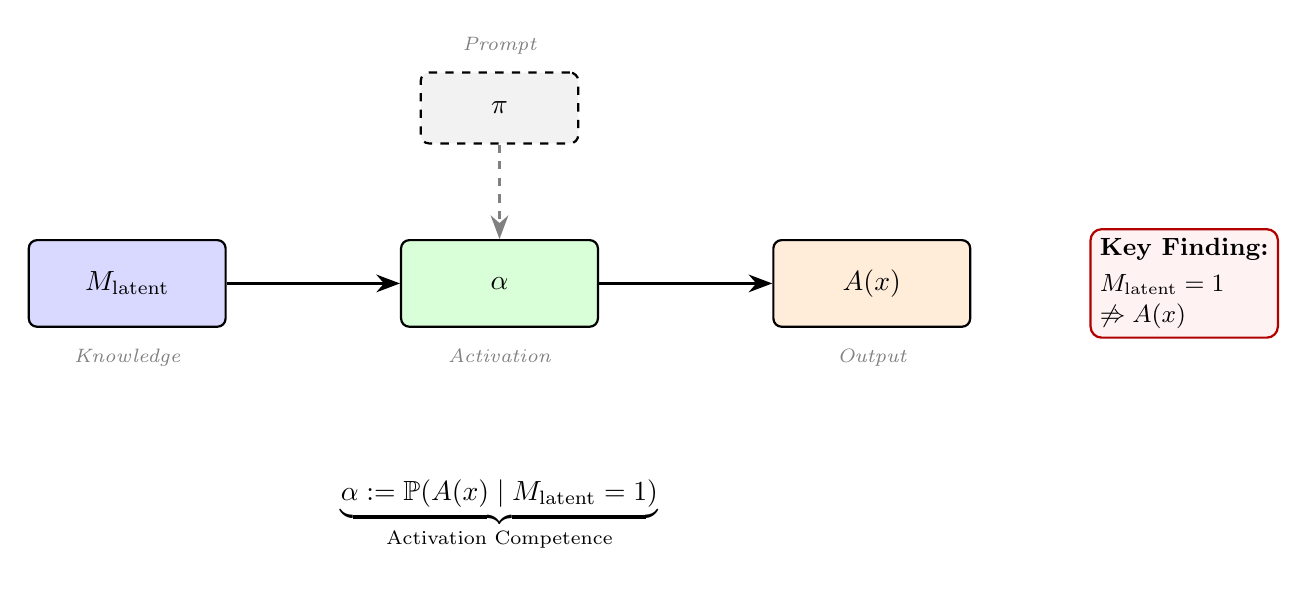
\begin{tikzpicture}[
    node distance=2.2cm,
    main/.style={rectangle, draw=black, thick, minimum width=2.5cm, minimum height=1.1cm, align=center, rounded corners=3pt},
    prompt/.style={rectangle, draw=black, thick, dashed, minimum width=2cm, minimum height=0.9cm, align=center, rounded corners=3pt, fill=gray!10},
    arrow/.style={-{Stealth[length=3mm]}, thick},
    note/.style={font=\scriptsize\itshape, text=gray}
]

% Main flow
\node[main, fill=blue!15] (M) {$M_{\text{latent}}$};
\node[main, fill=green!15, right=of M] (alpha) {$\alpha$};
\node[main, fill=orange!15, right=of alpha] (A) {$A(x)$};

% Prompt
\node[prompt, above=1.2cm of alpha] (pi) {$\pi$};

% Arrows
\draw[arrow] (M) -- (alpha);
\draw[arrow] (alpha) -- (A);
\draw[arrow, dashed, gray] (pi) -- (alpha);

% Labels
\node[note, below=0.15cm of M] {Knowledge};
\node[note, below=0.15cm of alpha] {Activation};
\node[note, below=0.15cm of A] {Output};
\node[note, above=0.1cm of pi] {Prompt};

% Equation
\node[below=1.8cm of alpha] {
    $\underbrace{\alpha := \mathbb{P}(A(x) \mid M_{\text{latent}} = 1)}_{\text{Activation Competence}}$
};

% Key insight box
\node[draw=red!70!black, thick, rounded corners, fill=red!5,
      right=1.5cm of A, align=left, font=\small] (insight) {
    \textbf{Key Finding:}\\[2pt]
    $M_{\text{latent}} = 1$\\
    $\not\Rightarrow A(x)$
};

\end{tikzpicture}
\caption{\textbf{Knowledge Activation Model.} The path from latent knowledge ($M_{\text{latent}}$) to correct output ($A(x)$) is mediated by activation competence ($\alpha$). Prompts ($\pi$) can modulate $\alpha$ but cannot create knowledge. The central finding is that knowledge availability does not guarantee knowledge application.}
\label{fig:main-model}
\end{figure}


% ============================================================================
% USAGE NOTES
% ============================================================================
%
% For paper inclusion, use Figure 5 (fig:main-model) as the main text figure.
% Other figures can go in appendix or supplementary material.
%
% Required packages:
% \usepackage{tikz}
% \usetikzlibrary{arrows.meta,positioning,shapes.geometric,calc,decorations.pathmorphing}
%
% To include in main paper:
% \begin{figure}[t]
%   \centering
%   \input{figures/activation-model.tikz}
%   \caption{...}
% \end{figure}
%

\end{document}
 or standalone compilation
% ============================================================================

\documentclass[11pt,a4paper]{article}
\usepackage[utf8]{inputenc}
\usepackage[T1]{fontenc}
\usepackage{amsmath,amssymb}
\usepackage{tikz}
\usetikzlibrary{arrows.meta,positioning,shapes.geometric,calc,decorations.pathmorphing}
\usepackage[margin=1in]{geometry}

\title{\textbf{Graphical Model: Knowledge Activation in LLMs}}
\author{BEATRIX Research Group}
\date{December 2025}

\begin{document}
\maketitle

% ============================================================================
\section{Main Figure: The Activation Gap}
% ============================================================================

\begin{figure}[h]
\centering
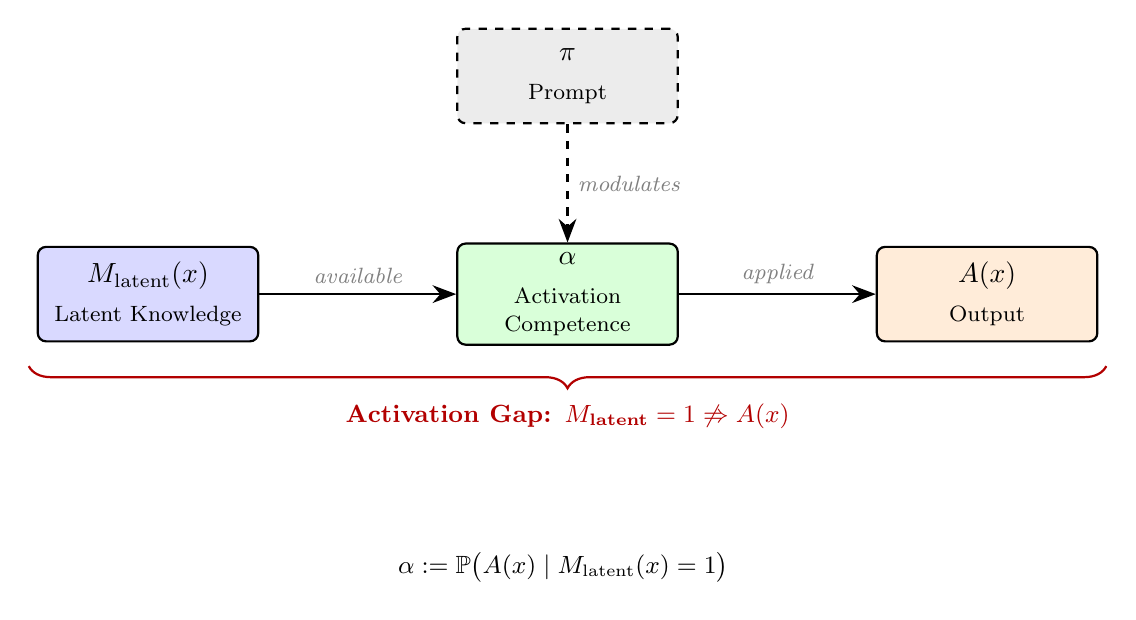
\begin{tikzpicture}[
    node distance=2.5cm,
    box/.style={rectangle, draw=black, thick, minimum width=2.8cm, minimum height=1.2cm, align=center, rounded corners=3pt},
    latent/.style={box, fill=blue!15},
    activation/.style={box, fill=green!15},
    output/.style={box, fill=orange!15},
    prompt/.style={box, fill=gray!15, dashed},
    arrow/.style={-{Stealth[length=3mm]}, thick},
    label/.style={font=\footnotesize\itshape, text=gray}
]

% Main pathway
\node[latent] (M) {$M_{\text{latent}}(x)$\\[2pt]\footnotesize Latent Knowledge};
\node[activation, right=of M] (alpha) {$\alpha$\\[2pt]\footnotesize Activation\\[-2pt]\footnotesize Competence};
\node[output, right=of alpha] (A) {$A(x)$\\[2pt]\footnotesize Output};

% Prompt node (influencing activation)
\node[prompt, above=1.5cm of alpha] (pi) {$\pi$\\[2pt]\footnotesize Prompt};

% Arrows
\draw[arrow] (M) -- (alpha) node[midway, above, label] {available};
\draw[arrow] (alpha) -- (A) node[midway, above, label] {applied};
\draw[arrow, dashed] (pi) -- (alpha) node[midway, right, label] {modulates};

% The Gap annotation
\draw[decorate, decoration={brace, amplitude=8pt, mirror}, thick, red!70!black]
    ($(M.south west)+(-0.1,-0.3)$) -- ($(A.south east)+(0.1,-0.3)$)
    node[midway, below=10pt, text=red!70!black, font=\small\bfseries] {Activation Gap: $M_{\text{latent}} = 1 \not\Rightarrow A(x)$};

% Probability annotation
\node[below=2.5cm of alpha, align=center, font=\small] {
    $\alpha := \mathbb{P}\big(A(x) \mid M_{\text{latent}}(x) = 1\big)$
};

\end{tikzpicture}
\caption{\textbf{The Knowledge Activation Model.} Latent knowledge $M_{\text{latent}}$ must pass through activation competence $\alpha$ before manifesting as correct output $A(x)$. The prompt $\pi$ modulates $\alpha$ but cannot create knowledge. The \textcolor{red!70!black}{activation gap} represents the central finding: knowledge availability does not imply knowledge use.}
\label{fig:activation-model}
\end{figure}


% ============================================================================
\section{Extended Figure: Decomposition and Prompt Effects}
% ============================================================================

\begin{figure}[h]
\centering
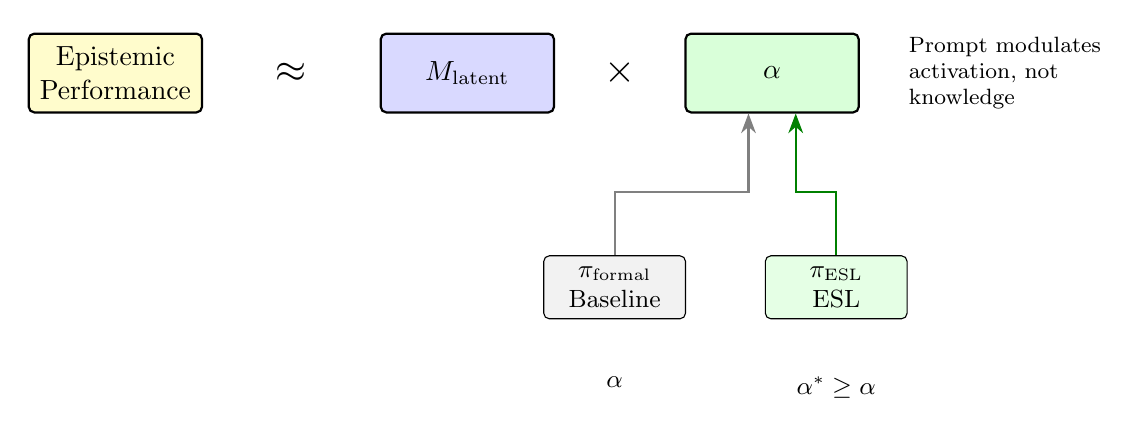
\begin{tikzpicture}[
    node distance=2cm,
    box/.style={rectangle, draw=black, thick, minimum width=2.2cm, minimum height=1cm, align=center, rounded corners=2pt},
    small/.style={rectangle, draw=black, minimum width=1.8cm, minimum height=0.8cm, align=center, rounded corners=2pt, font=\small},
    arrow/.style={-{Stealth[length=2.5mm]}, thick},
    eq/.style={font=\Large}
]

% Performance decomposition
\node[box, fill=yellow!20] (perf) {Epistemic\\Performance};
\node[eq, right=0.8cm of perf] (eq1) {$\approx$};
\node[box, fill=blue!15, right=0.8cm of eq1] (M2) {$M_{\text{latent}}$};
\node[eq, right=0.5cm of M2] (times) {$\times$};
\node[box, fill=green!15, right=0.5cm of times] (alpha2) {$\alpha$};

% Prompt conditions below
\node[small, fill=gray!10, below=1.8cm of alpha2, xshift=-2cm] (baseline) {$\pi_{\text{formal}}$\\Baseline};
\node[small, fill=green!10, right=1cm of baseline] (esl) {$\pi_{\text{ESL}}$\\ESL};

% Alpha values
\node[below=0.6cm of baseline, font=\small] (a1) {$\alpha$};
\node[below=0.6cm of esl, font=\small] (a2) {$\alpha^* \geq \alpha$};

% Arrows from prompts to alpha
\draw[arrow, gray] (baseline.north) -- ++(0,0.8) -| ($(alpha2.south)+(-0.3,0)$);
\draw[arrow, green!50!black] (esl.north) -- ++(0,0.8) -| ($(alpha2.south)+(0.3,0)$);

% Annotation
\node[right=0.5cm of alpha2, align=left, font=\footnotesize] {
    Prompt modulates\\
    activation, not\\
    knowledge
};

\end{tikzpicture}
\caption{\textbf{Performance Decomposition.} Epistemic performance decomposes into latent knowledge times activation competence. Different prompts ($\pi_{\text{formal}}$ vs.\ $\pi_{\text{ESL}}$) yield different activation levels, with ESL achieving $\alpha^* \geq \alpha$.}
\label{fig:decomposition}
\end{figure}


% ============================================================================
\section{Comparative Figure: Model Profiles}
% ============================================================================

\begin{figure}[h]
\centering
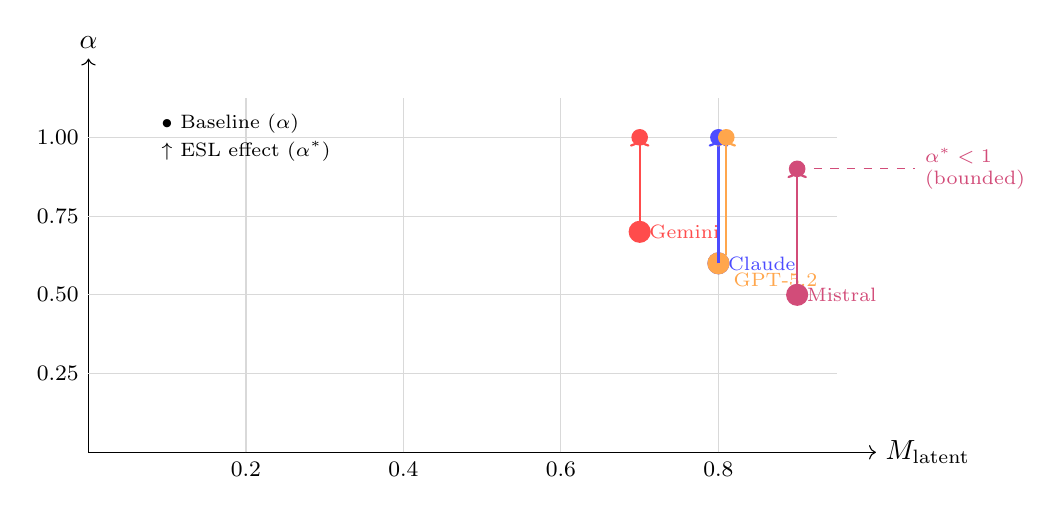
\begin{tikzpicture}[
    bar/.style={thick},
    label/.style={font=\footnotesize}
]

% Axes
\draw[->] (0,0) -- (10,0) node[right] {$M_{\text{latent}}$};
\draw[->] (0,0) -- (0,5) node[above] {$\alpha$};

% Grid
\foreach \x in {2,4,6,8} {
    \draw[gray!30] (\x,0) -- (\x,4.5);
}
\foreach \y in {1,2,3,4} {
    \draw[gray!30] (0,\y) -- (9.5,\y);
}

% Axis labels
\node[label, below] at (2,0) {0.2};
\node[label, below] at (4,0) {0.4};
\node[label, below] at (6,0) {0.6};
\node[label, below] at (8,0) {0.8};
\node[label, left] at (0,1) {0.25};
\node[label, left] at (0,2) {0.50};
\node[label, left] at (0,3) {0.75};
\node[label, left] at (0,4) {1.00};

% Model points (Baseline)
\fill[blue!70] (8,2.4) circle (4pt) node[right, font=\scriptsize] {Claude};
\fill[red!70] (7,2.8) circle (4pt) node[right, font=\scriptsize] {Gemini};
\fill[orange!70] (8,2.4) circle (4pt) node[below right, font=\scriptsize, xshift=2pt] {GPT-5.2};
\fill[purple!70] (9,2) circle (4pt) node[right, font=\scriptsize] {Mistral};

% Arrows to ESL positions
\draw[->, blue!70, thick] (8,2.4) -- (8,4);
\draw[->, red!70, thick] (7,2.8) -- (7,4);
\draw[->, orange!70, thick] (8.1,2.5) -- (8.1,4);
\draw[->, purple!70, thick] (9,2) -- (9,3.6);

% ESL points
\fill[blue!70] (8,4) circle (3pt);
\fill[red!70] (7,4) circle (3pt);
\fill[orange!70] (8.1,4) circle (3pt);
\fill[purple!70] (9,3.6) circle (3pt);

% Legend
\node[font=\scriptsize, align=left] at (2,4) {
    $\bullet$ Baseline ($\alpha$)\\[2pt]
    $\uparrow$ ESL effect ($\alpha^*$)
};

% Annotation for Mistral
\draw[purple!70, dashed] (9,3.6) -- (10.5,3.6) node[right, font=\scriptsize, align=left] {$\alpha^* < 1$\\(bounded)};

\end{tikzpicture}
\caption{\textbf{Cross-Model Activation Profiles.} All models have high latent knowledge ($M_{\text{latent}} \approx 0.8$--$0.9$), but vary in baseline activation ($\alpha = 0.50$--$0.70$). ESL prompting increases $\alpha$ to $\alpha^*$, with most models reaching 1.00. Mistral shows bounded activation ($\alpha^* = 0.90 < 1$), indicating intrinsic limitations.}
\label{fig:model-profiles}
\end{figure}


% ============================================================================
\section{Conceptual Figure: Hallucination as Activation Failure}
% ============================================================================

\begin{figure}[h]
\centering
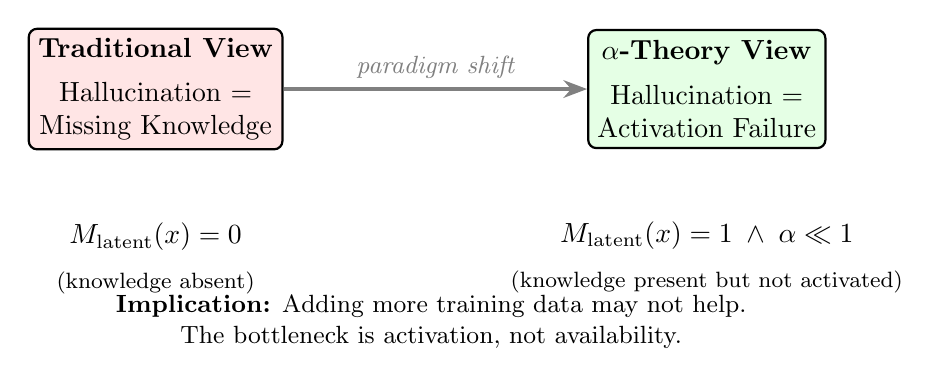
\begin{tikzpicture}[
    box/.style={rectangle, draw=black, thick, minimum width=3cm, minimum height=1.5cm, align=center, rounded corners=3pt},
    arrow/.style={-{Stealth[length=3mm]}, thick}
]

% Two scenarios side by side
% Scenario 1: Traditional view
\node[box, fill=red!10] (trad) at (0,0) {\textbf{Traditional View}\\[4pt]Hallucination =\\Missing Knowledge};

% Scenario 2: Alpha view
\node[box, fill=green!10] (alpha) at (7,0) {\textbf{$\alpha$-Theory View}\\[4pt]Hallucination =\\Activation Failure};

% Formulas below
\node[below=0.8cm of trad, align=center] {
    $M_{\text{latent}}(x) = 0$\\[4pt]
    \footnotesize (knowledge absent)
};

\node[below=0.8cm of alpha, align=center] {
    $M_{\text{latent}}(x) = 1 \;\land\; \alpha \ll 1$\\[4pt]
    \footnotesize (knowledge present but not activated)
};

% Arrow between views
\draw[arrow, very thick, gray] (trad) -- (alpha) node[midway, above, font=\small\itshape] {paradigm shift};

% Implication
\node[below=2.5cm of $(trad)!0.5!(alpha)$, align=center, font=\small] {
    \textbf{Implication:} Adding more training data may not help.\\
    The bottleneck is activation, not availability.
};

\end{tikzpicture}
\caption{\textbf{Reframing Hallucination.} The traditional view attributes hallucination to missing knowledge. The $\alpha$-theory reframes it as activation failure: the model possesses the relevant knowledge but fails to apply it during generation.}
\label{fig:hallucination-reframe}
\end{figure}


% ============================================================================
\section{Paper-Ready Single Figure (Recommended for Main Text)}
% ============================================================================

\begin{figure}[h]
\centering
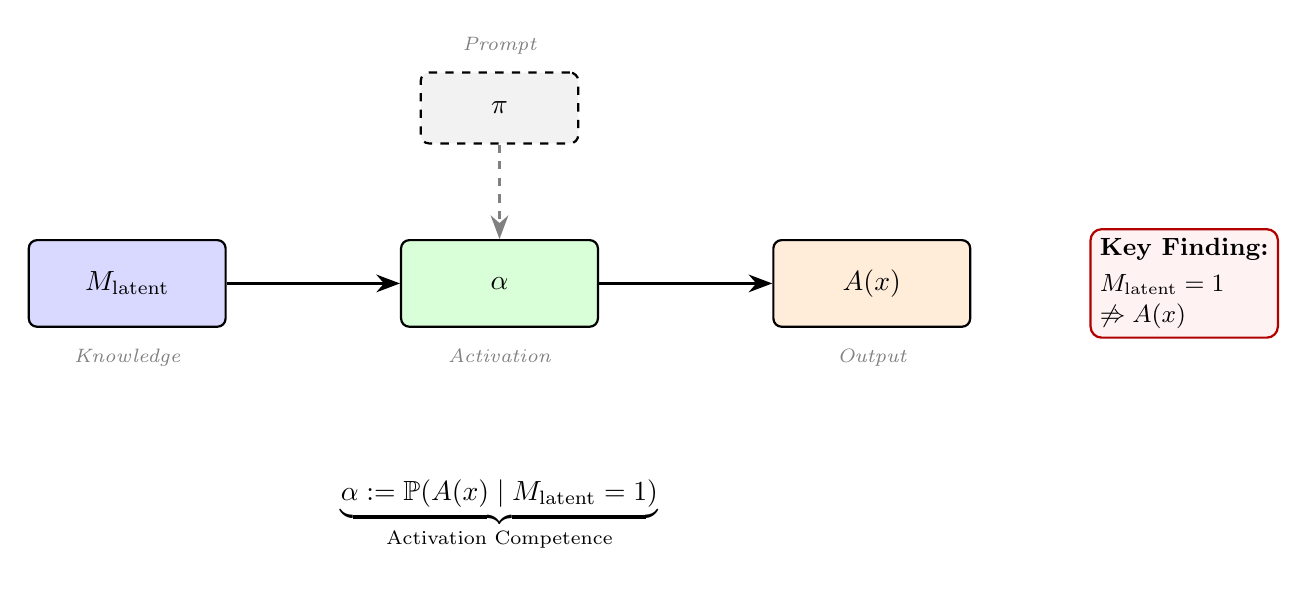
\begin{tikzpicture}[
    node distance=2.2cm,
    main/.style={rectangle, draw=black, thick, minimum width=2.5cm, minimum height=1.1cm, align=center, rounded corners=3pt},
    prompt/.style={rectangle, draw=black, thick, dashed, minimum width=2cm, minimum height=0.9cm, align=center, rounded corners=3pt, fill=gray!10},
    arrow/.style={-{Stealth[length=3mm]}, thick},
    note/.style={font=\scriptsize\itshape, text=gray}
]

% Main flow
\node[main, fill=blue!15] (M) {$M_{\text{latent}}$};
\node[main, fill=green!15, right=of M] (alpha) {$\alpha$};
\node[main, fill=orange!15, right=of alpha] (A) {$A(x)$};

% Prompt
\node[prompt, above=1.2cm of alpha] (pi) {$\pi$};

% Arrows
\draw[arrow] (M) -- (alpha);
\draw[arrow] (alpha) -- (A);
\draw[arrow, dashed, gray] (pi) -- (alpha);

% Labels
\node[note, below=0.15cm of M] {Knowledge};
\node[note, below=0.15cm of alpha] {Activation};
\node[note, below=0.15cm of A] {Output};
\node[note, above=0.1cm of pi] {Prompt};

% Equation
\node[below=1.8cm of alpha] {
    $\underbrace{\alpha := \mathbb{P}(A(x) \mid M_{\text{latent}} = 1)}_{\text{Activation Competence}}$
};

% Key insight box
\node[draw=red!70!black, thick, rounded corners, fill=red!5,
      right=1.5cm of A, align=left, font=\small] (insight) {
    \textbf{Key Finding:}\\[2pt]
    $M_{\text{latent}} = 1$\\
    $\not\Rightarrow A(x)$
};

\end{tikzpicture}
\caption{\textbf{Knowledge Activation Model.} The path from latent knowledge ($M_{\text{latent}}$) to correct output ($A(x)$) is mediated by activation competence ($\alpha$). Prompts ($\pi$) can modulate $\alpha$ but cannot create knowledge. The central finding is that knowledge availability does not guarantee knowledge application.}
\label{fig:main-model}
\end{figure}


% ============================================================================
% USAGE NOTES
% ============================================================================
%
% For paper inclusion, use Figure 5 (fig:main-model) as the main text figure.
% Other figures can go in appendix or supplementary material.
%
% Required packages:
% \usepackage{tikz}
% \usetikzlibrary{arrows.meta,positioning,shapes.geometric,calc,decorations.pathmorphing}
%
% To include in main paper:
% \begin{figure}[t]
%   \centering
%   \input{figures/activation-model.tikz}
%   \caption{...}
% \end{figure}
%

\end{document}
 or standalone compilation
% ============================================================================

\documentclass[11pt,a4paper]{article}
\usepackage[utf8]{inputenc}
\usepackage[T1]{fontenc}
\usepackage{amsmath,amssymb}
\usepackage{tikz}
\usetikzlibrary{arrows.meta,positioning,shapes.geometric,calc,decorations.pathmorphing}
\usepackage[margin=1in]{geometry}

\title{\textbf{Graphical Model: Knowledge Activation in LLMs}}
\author{BEATRIX Research Group}
\date{December 2025}

\begin{document}
\maketitle

% ============================================================================
\section{Main Figure: The Activation Gap}
% ============================================================================

\begin{figure}[h]
\centering
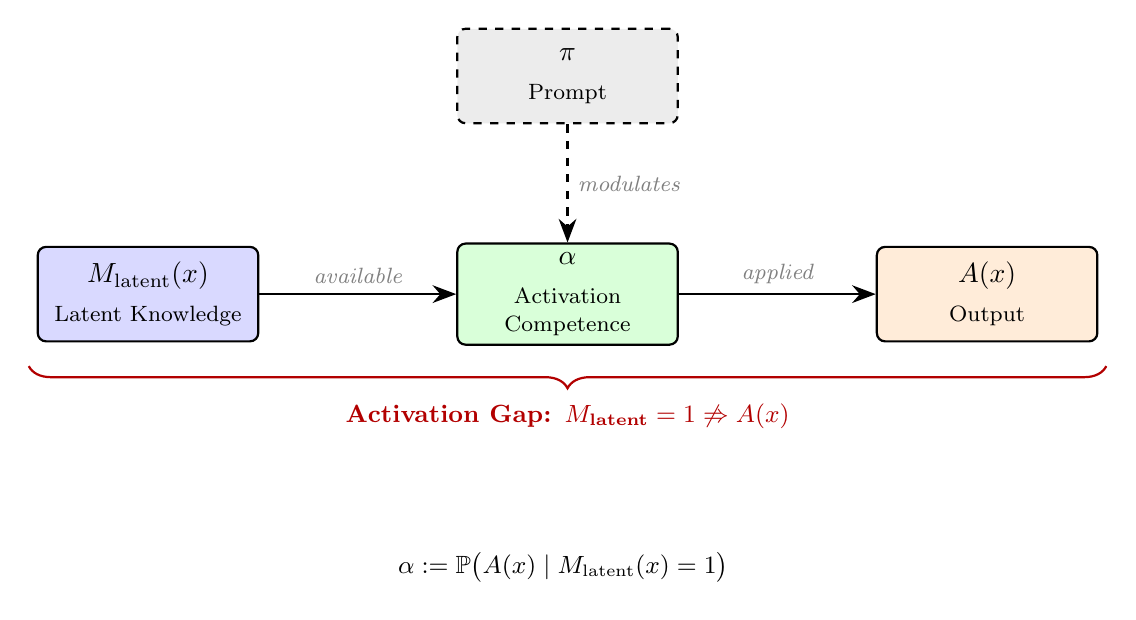
\begin{tikzpicture}[
    node distance=2.5cm,
    box/.style={rectangle, draw=black, thick, minimum width=2.8cm, minimum height=1.2cm, align=center, rounded corners=3pt},
    latent/.style={box, fill=blue!15},
    activation/.style={box, fill=green!15},
    output/.style={box, fill=orange!15},
    prompt/.style={box, fill=gray!15, dashed},
    arrow/.style={-{Stealth[length=3mm]}, thick},
    label/.style={font=\footnotesize\itshape, text=gray}
]

% Main pathway
\node[latent] (M) {$M_{\text{latent}}(x)$\\[2pt]\footnotesize Latent Knowledge};
\node[activation, right=of M] (alpha) {$\alpha$\\[2pt]\footnotesize Activation\\[-2pt]\footnotesize Competence};
\node[output, right=of alpha] (A) {$A(x)$\\[2pt]\footnotesize Output};

% Prompt node (influencing activation)
\node[prompt, above=1.5cm of alpha] (pi) {$\pi$\\[2pt]\footnotesize Prompt};

% Arrows
\draw[arrow] (M) -- (alpha) node[midway, above, label] {available};
\draw[arrow] (alpha) -- (A) node[midway, above, label] {applied};
\draw[arrow, dashed] (pi) -- (alpha) node[midway, right, label] {modulates};

% The Gap annotation
\draw[decorate, decoration={brace, amplitude=8pt, mirror}, thick, red!70!black]
    ($(M.south west)+(-0.1,-0.3)$) -- ($(A.south east)+(0.1,-0.3)$)
    node[midway, below=10pt, text=red!70!black, font=\small\bfseries] {Activation Gap: $M_{\text{latent}} = 1 \not\Rightarrow A(x)$};

% Probability annotation
\node[below=2.5cm of alpha, align=center, font=\small] {
    $\alpha := \mathbb{P}\big(A(x) \mid M_{\text{latent}}(x) = 1\big)$
};

\end{tikzpicture}
\caption{\textbf{The Knowledge Activation Model.} Latent knowledge $M_{\text{latent}}$ must pass through activation competence $\alpha$ before manifesting as correct output $A(x)$. The prompt $\pi$ modulates $\alpha$ but cannot create knowledge. The \textcolor{red!70!black}{activation gap} represents the central finding: knowledge availability does not imply knowledge use.}
\label{fig:activation-model}
\end{figure}


% ============================================================================
\section{Extended Figure: Decomposition and Prompt Effects}
% ============================================================================

\begin{figure}[h]
\centering
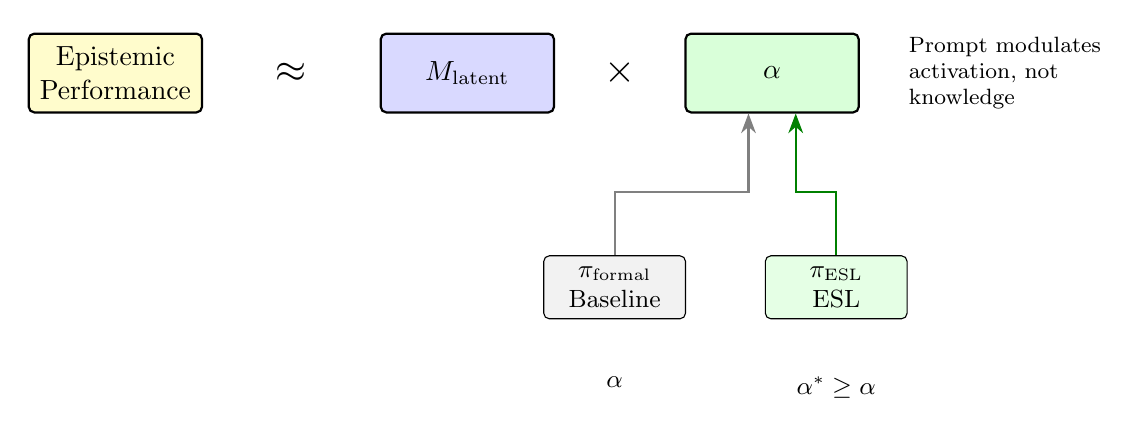
\begin{tikzpicture}[
    node distance=2cm,
    box/.style={rectangle, draw=black, thick, minimum width=2.2cm, minimum height=1cm, align=center, rounded corners=2pt},
    small/.style={rectangle, draw=black, minimum width=1.8cm, minimum height=0.8cm, align=center, rounded corners=2pt, font=\small},
    arrow/.style={-{Stealth[length=2.5mm]}, thick},
    eq/.style={font=\Large}
]

% Performance decomposition
\node[box, fill=yellow!20] (perf) {Epistemic\\Performance};
\node[eq, right=0.8cm of perf] (eq1) {$\approx$};
\node[box, fill=blue!15, right=0.8cm of eq1] (M2) {$M_{\text{latent}}$};
\node[eq, right=0.5cm of M2] (times) {$\times$};
\node[box, fill=green!15, right=0.5cm of times] (alpha2) {$\alpha$};

% Prompt conditions below
\node[small, fill=gray!10, below=1.8cm of alpha2, xshift=-2cm] (baseline) {$\pi_{\text{formal}}$\\Baseline};
\node[small, fill=green!10, right=1cm of baseline] (esl) {$\pi_{\text{ESL}}$\\ESL};

% Alpha values
\node[below=0.6cm of baseline, font=\small] (a1) {$\alpha$};
\node[below=0.6cm of esl, font=\small] (a2) {$\alpha^* \geq \alpha$};

% Arrows from prompts to alpha
\draw[arrow, gray] (baseline.north) -- ++(0,0.8) -| ($(alpha2.south)+(-0.3,0)$);
\draw[arrow, green!50!black] (esl.north) -- ++(0,0.8) -| ($(alpha2.south)+(0.3,0)$);

% Annotation
\node[right=0.5cm of alpha2, align=left, font=\footnotesize] {
    Prompt modulates\\
    activation, not\\
    knowledge
};

\end{tikzpicture}
\caption{\textbf{Performance Decomposition.} Epistemic performance decomposes into latent knowledge times activation competence. Different prompts ($\pi_{\text{formal}}$ vs.\ $\pi_{\text{ESL}}$) yield different activation levels, with ESL achieving $\alpha^* \geq \alpha$.}
\label{fig:decomposition}
\end{figure}


% ============================================================================
\section{Comparative Figure: Model Profiles}
% ============================================================================

\begin{figure}[h]
\centering
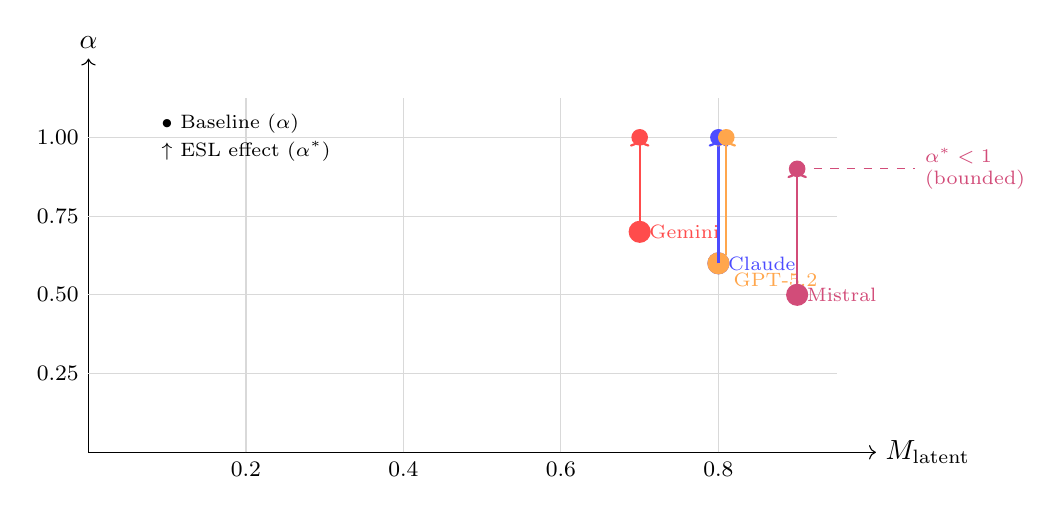
\begin{tikzpicture}[
    bar/.style={thick},
    label/.style={font=\footnotesize}
]

% Axes
\draw[->] (0,0) -- (10,0) node[right] {$M_{\text{latent}}$};
\draw[->] (0,0) -- (0,5) node[above] {$\alpha$};

% Grid
\foreach \x in {2,4,6,8} {
    \draw[gray!30] (\x,0) -- (\x,4.5);
}
\foreach \y in {1,2,3,4} {
    \draw[gray!30] (0,\y) -- (9.5,\y);
}

% Axis labels
\node[label, below] at (2,0) {0.2};
\node[label, below] at (4,0) {0.4};
\node[label, below] at (6,0) {0.6};
\node[label, below] at (8,0) {0.8};
\node[label, left] at (0,1) {0.25};
\node[label, left] at (0,2) {0.50};
\node[label, left] at (0,3) {0.75};
\node[label, left] at (0,4) {1.00};

% Model points (Baseline)
\fill[blue!70] (8,2.4) circle (4pt) node[right, font=\scriptsize] {Claude};
\fill[red!70] (7,2.8) circle (4pt) node[right, font=\scriptsize] {Gemini};
\fill[orange!70] (8,2.4) circle (4pt) node[below right, font=\scriptsize, xshift=2pt] {GPT-5.2};
\fill[purple!70] (9,2) circle (4pt) node[right, font=\scriptsize] {Mistral};

% Arrows to ESL positions
\draw[->, blue!70, thick] (8,2.4) -- (8,4);
\draw[->, red!70, thick] (7,2.8) -- (7,4);
\draw[->, orange!70, thick] (8.1,2.5) -- (8.1,4);
\draw[->, purple!70, thick] (9,2) -- (9,3.6);

% ESL points
\fill[blue!70] (8,4) circle (3pt);
\fill[red!70] (7,4) circle (3pt);
\fill[orange!70] (8.1,4) circle (3pt);
\fill[purple!70] (9,3.6) circle (3pt);

% Legend
\node[font=\scriptsize, align=left] at (2,4) {
    $\bullet$ Baseline ($\alpha$)\\[2pt]
    $\uparrow$ ESL effect ($\alpha^*$)
};

% Annotation for Mistral
\draw[purple!70, dashed] (9,3.6) -- (10.5,3.6) node[right, font=\scriptsize, align=left] {$\alpha^* < 1$\\(bounded)};

\end{tikzpicture}
\caption{\textbf{Cross-Model Activation Profiles.} All models have high latent knowledge ($M_{\text{latent}} \approx 0.8$--$0.9$), but vary in baseline activation ($\alpha = 0.50$--$0.70$). ESL prompting increases $\alpha$ to $\alpha^*$, with most models reaching 1.00. Mistral shows bounded activation ($\alpha^* = 0.90 < 1$), indicating intrinsic limitations.}
\label{fig:model-profiles}
\end{figure}


% ============================================================================
\section{Conceptual Figure: Hallucination as Activation Failure}
% ============================================================================

\begin{figure}[h]
\centering
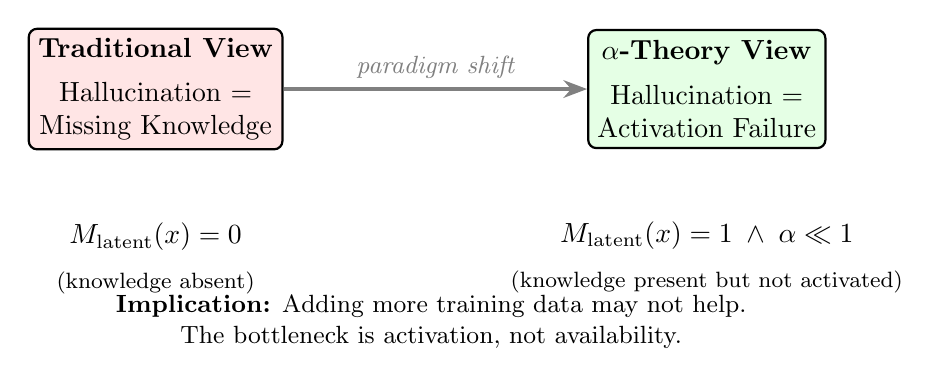
\begin{tikzpicture}[
    box/.style={rectangle, draw=black, thick, minimum width=3cm, minimum height=1.5cm, align=center, rounded corners=3pt},
    arrow/.style={-{Stealth[length=3mm]}, thick}
]

% Two scenarios side by side
% Scenario 1: Traditional view
\node[box, fill=red!10] (trad) at (0,0) {\textbf{Traditional View}\\[4pt]Hallucination =\\Missing Knowledge};

% Scenario 2: Alpha view
\node[box, fill=green!10] (alpha) at (7,0) {\textbf{$\alpha$-Theory View}\\[4pt]Hallucination =\\Activation Failure};

% Formulas below
\node[below=0.8cm of trad, align=center] {
    $M_{\text{latent}}(x) = 0$\\[4pt]
    \footnotesize (knowledge absent)
};

\node[below=0.8cm of alpha, align=center] {
    $M_{\text{latent}}(x) = 1 \;\land\; \alpha \ll 1$\\[4pt]
    \footnotesize (knowledge present but not activated)
};

% Arrow between views
\draw[arrow, very thick, gray] (trad) -- (alpha) node[midway, above, font=\small\itshape] {paradigm shift};

% Implication
\node[below=2.5cm of $(trad)!0.5!(alpha)$, align=center, font=\small] {
    \textbf{Implication:} Adding more training data may not help.\\
    The bottleneck is activation, not availability.
};

\end{tikzpicture}
\caption{\textbf{Reframing Hallucination.} The traditional view attributes hallucination to missing knowledge. The $\alpha$-theory reframes it as activation failure: the model possesses the relevant knowledge but fails to apply it during generation.}
\label{fig:hallucination-reframe}
\end{figure}


% ============================================================================
\section{Paper-Ready Single Figure (Recommended for Main Text)}
% ============================================================================

\begin{figure}[h]
\centering
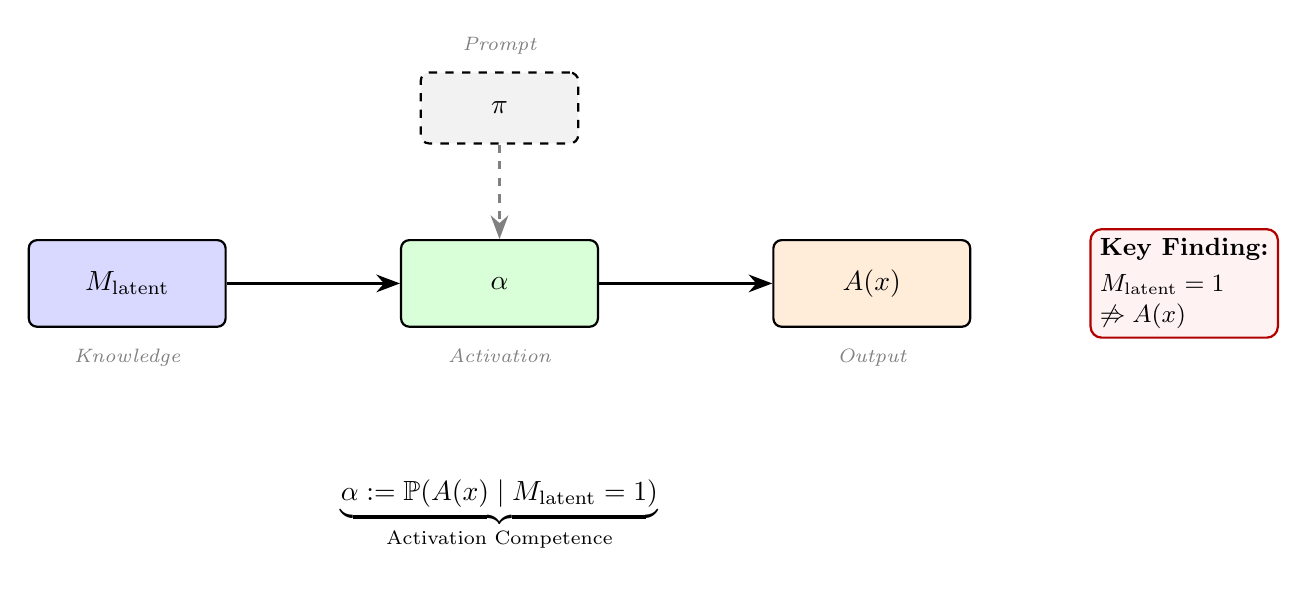
\begin{tikzpicture}[
    node distance=2.2cm,
    main/.style={rectangle, draw=black, thick, minimum width=2.5cm, minimum height=1.1cm, align=center, rounded corners=3pt},
    prompt/.style={rectangle, draw=black, thick, dashed, minimum width=2cm, minimum height=0.9cm, align=center, rounded corners=3pt, fill=gray!10},
    arrow/.style={-{Stealth[length=3mm]}, thick},
    note/.style={font=\scriptsize\itshape, text=gray}
]

% Main flow
\node[main, fill=blue!15] (M) {$M_{\text{latent}}$};
\node[main, fill=green!15, right=of M] (alpha) {$\alpha$};
\node[main, fill=orange!15, right=of alpha] (A) {$A(x)$};

% Prompt
\node[prompt, above=1.2cm of alpha] (pi) {$\pi$};

% Arrows
\draw[arrow] (M) -- (alpha);
\draw[arrow] (alpha) -- (A);
\draw[arrow, dashed, gray] (pi) -- (alpha);

% Labels
\node[note, below=0.15cm of M] {Knowledge};
\node[note, below=0.15cm of alpha] {Activation};
\node[note, below=0.15cm of A] {Output};
\node[note, above=0.1cm of pi] {Prompt};

% Equation
\node[below=1.8cm of alpha] {
    $\underbrace{\alpha := \mathbb{P}(A(x) \mid M_{\text{latent}} = 1)}_{\text{Activation Competence}}$
};

% Key insight box
\node[draw=red!70!black, thick, rounded corners, fill=red!5,
      right=1.5cm of A, align=left, font=\small] (insight) {
    \textbf{Key Finding:}\\[2pt]
    $M_{\text{latent}} = 1$\\
    $\not\Rightarrow A(x)$
};

\end{tikzpicture}
\caption{\textbf{Knowledge Activation Model.} The path from latent knowledge ($M_{\text{latent}}$) to correct output ($A(x)$) is mediated by activation competence ($\alpha$). Prompts ($\pi$) can modulate $\alpha$ but cannot create knowledge. The central finding is that knowledge availability does not guarantee knowledge application.}
\label{fig:main-model}
\end{figure}


% ============================================================================
% USAGE NOTES
% ============================================================================
%
% For paper inclusion, use Figure 5 (fig:main-model) as the main text figure.
% Other figures can go in appendix or supplementary material.
%
% Required packages:
% \usepackage{tikz}
% \usetikzlibrary{arrows.meta,positioning,shapes.geometric,calc,decorations.pathmorphing}
%
% To include in main paper:
% \begin{figure}[t]
%   \centering
%   \input{figures/activation-model.tikz}
%   \caption{...}
% \end{figure}
%

\end{document}
